\chapter{Appendices}
\label{ch:phys-appx}


%% Neutrino Interactions and Uncertainties Appendix 
%% Assigned to: Kevin McFarland with Kendall Mahn and DuneReweight team 
%\section{Appendiz: Neutrino Interactions and Uncertainties}\label{sec:nu-osc-11} \label{sec:physics-lbnosc-nuint-app}
%{\it Assigned to:} {\bf Kevin McFarland}

%% Near Detector and Uncertainties Appendix 
%% Assigned to: Chris Marshall with Mike Kordorsky and Steven Manly 
%\section{Appendix: Near Detector and Uncertainties}\label{sec:nu-osc-12}\label{sec:physics-lbnosc-ND-app}
%{\it Assigned to:} {\bf Chris Marshall} 

%%%%%%%%%%%%%%%%%%%%%%%%%%%%%%%%%%%%%%%%%%%%%%%%%%%%%%%%%%%%%%%%
\section{Tools and Methods}
\label{sec:tools-appendix}

\subsection{Additional Simulation Details}

%%%%%%%%%%%%%%%%%%%%%%%%%%%%%%%%%%%%%%%%%%%%%%%%%%%%%%%%%%%%%%%%
\subsubsection{Additional Flux Modeling Details}
\label{sec:tools-app-flx}

\subsubsection{Off-axis Neutrino Flux and Uncertainties}
\label{sec:tools-app-flx-offaxis}

The neutrino flux has a broad angular distribution and extends outward at the \dword{nd} hall. At an ``off-axis'' angle relative to the initial beam direction, the subsequent neutrino energy spectrum is narrower and peaked at a lower energy than the on-axis spectrum.
The relationship between the parent pion energy and neutrino energy is shown in Figure~\ref{fig:OAAFluxFigs}.  At \SI{575}{m}, the location of the \dword{nd} hall, a lateral shift of \SI{1}{m} corresponds to approximately a \ang{0.1} change in off-axis angle.

\begin{dunefigure}[$\nu$ energy as  function of parent pion energy for different angles away from the pion momentum vector]{fig:OAAFluxFigs}
{(left) The neutrino energy as a function of parent pion energy for different angles away from the pion momentum vector. Figure from Ref.~\cite{Duffy:2016owt}. (right) The DUNE near detector flux predictions over a range of off-axis positions for a near detector at \SI{575}{m} downstream of the target station. }
%is subfig package included? I don't think subfloat is working (ZP)
%  \subfloat[C][Off-axis pion decay kinematics]{
    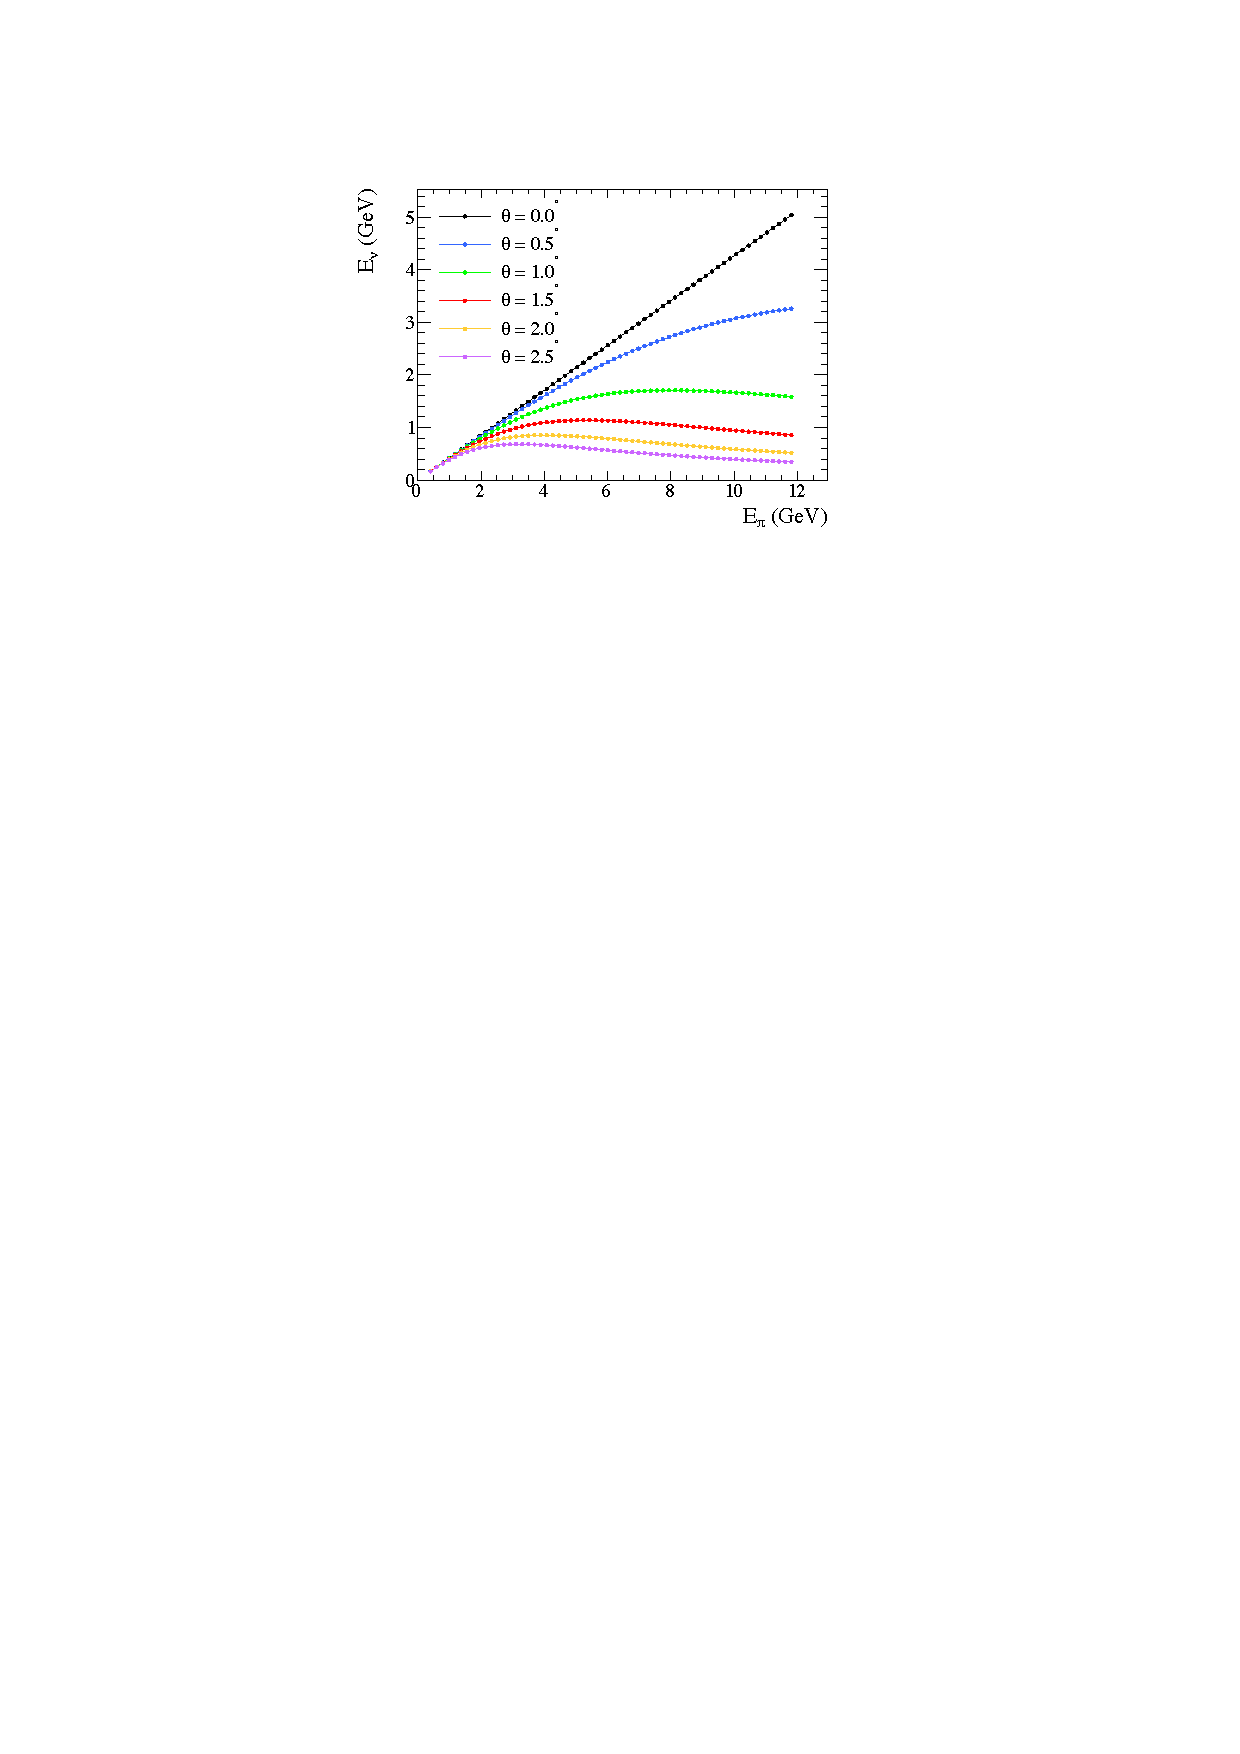
\includegraphics[width=0.4\textwidth]{OATrick}
%    \label{fig:OATrick}
%  }
%  \subfloat[][DUNE near detector flux predictions]{
    \raisebox{0.5em}{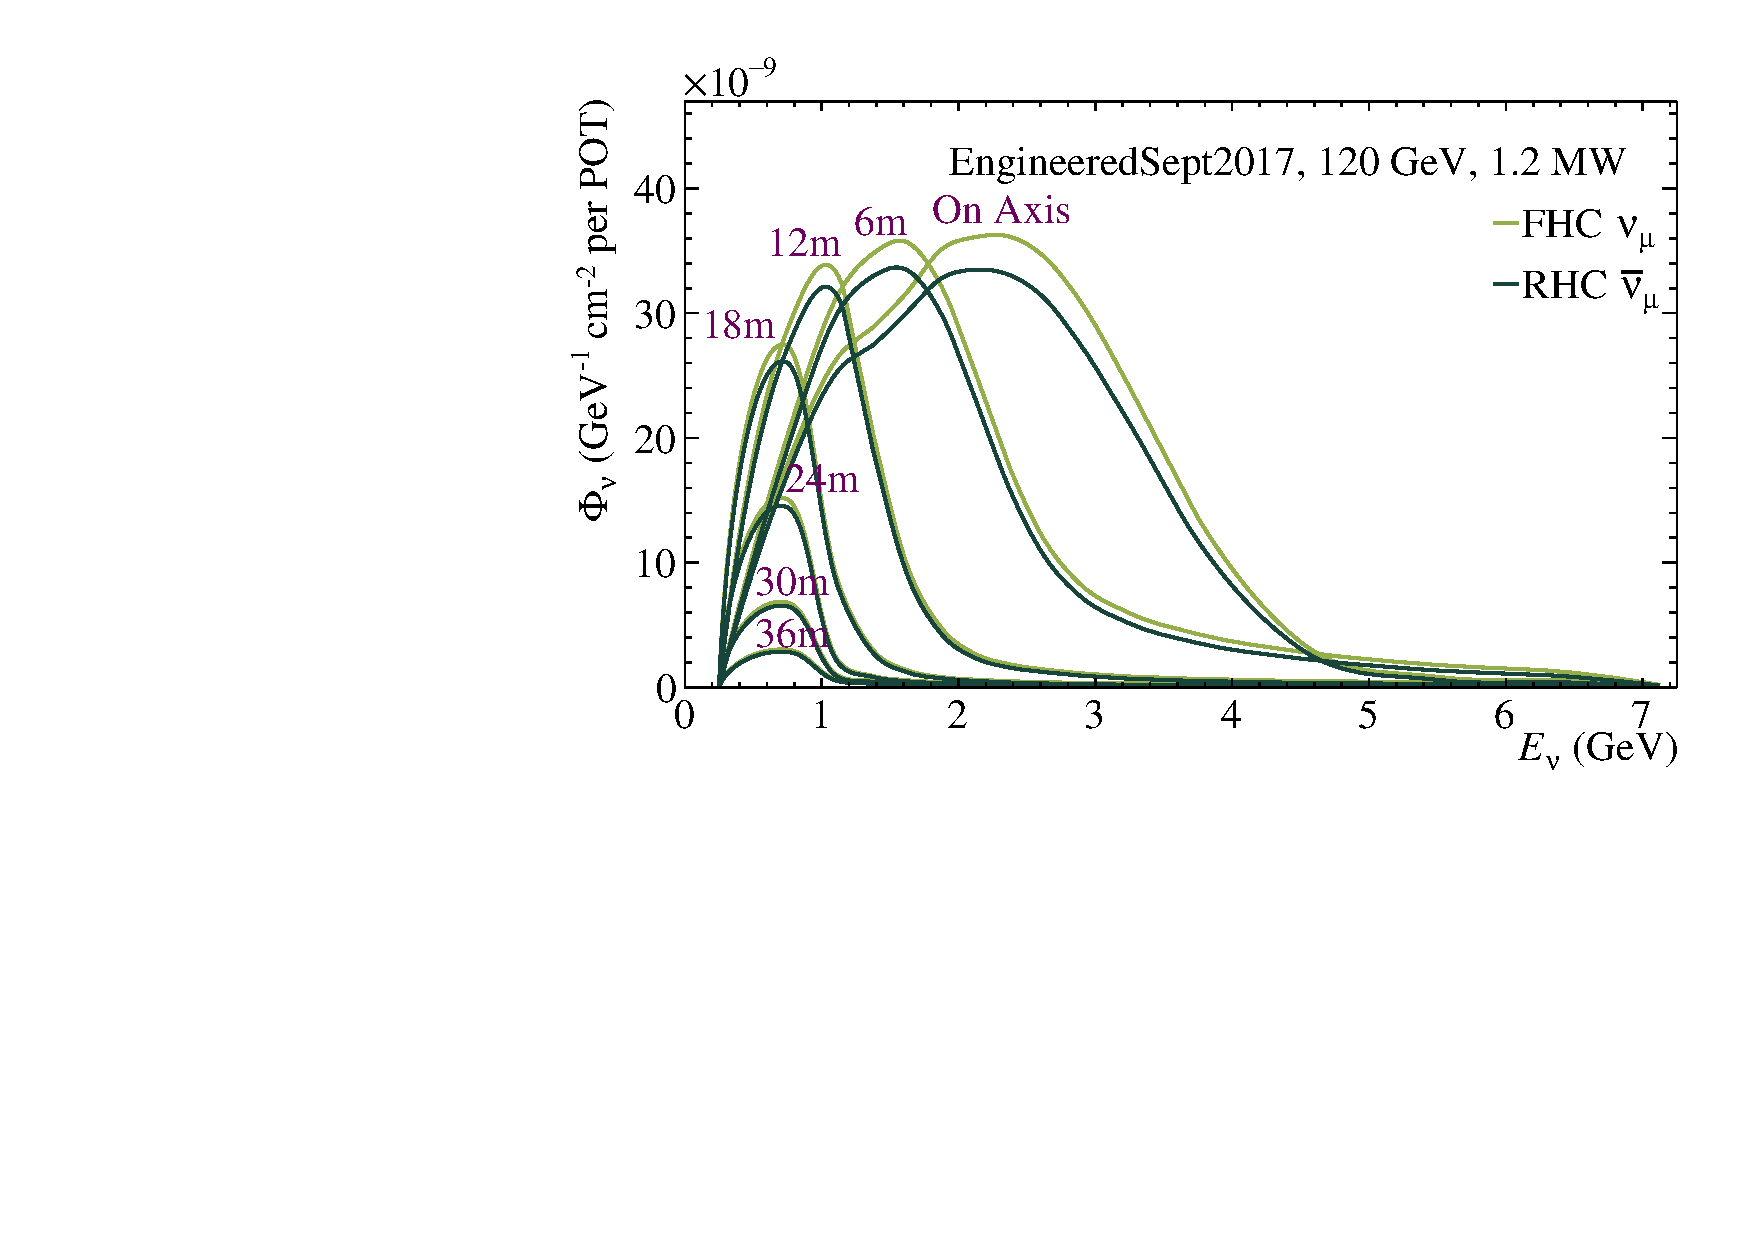
\includegraphics[width=0.45\textwidth]{OffAxisFluxes_1D}}
%    \label{fig:OffAxisFluxes_1D}
%  }
\end{dunefigure}

The intrinsic neutrino flavor content of the beam varies with off-axis angle. Figure~\ref{fig:OffAxisFluxes_1D_AllSpec} shows the neutrino-mode and anti-neutrino-mode predictions for the four neutrino flavors at the on-axis position, and a moderately off-axis position. At the \SI{30}{m} position, a second, smaller energy peak at approximately \SI{4}{\GeV} is due to the charged kaon neutrino parents. 
%As both the pion and kaon-parent peaks are significantly narrower in observed neutrino energy at greater off-axis angle, this which may allow for off-axis kaon-parent analyses.

%\fixme{Fig~\ref{fig:OffAxisFluxes_1D_AllSpec} is partly redundant with earlier figure, nice if it can be merged? }
%ZP: Changed previous plot. Unlike this one it shows all of the neutrino species broken by parent and it is on linear scale. Here useful to have comparison on vs offaxis and on log scale
\begin{dunefigure}[The predicted muon neutrino energy spectra at two near detector positions, on axis and \SI{30}{m} off axis.]{fig:OffAxisFluxes_1D_AllSpec}
{The predicted muon neutrino energy spectra at two \dword{nd} positions, on axis and \SI{30}{m} off axis. (a) The predicted neutrino flavor-content of the neutrino-mode (FHC) and anti-neutrino-mode (RHC) beam. (b) The neutrino-mode, muon-flavor predicted flux, separated by the particle that decayed to produce the neutrino. The off-axis spectrum displays a double peak structure due to charged kaon parent decay kinematics. The on-axis kaon-peak occurs at higher neutrino energy and will have a significantly broader energy spread. Top: Beam neutrino flavor content, middle: Beam neutrino flavor content; bottom: Beam neutrino decay-parent species}
   % 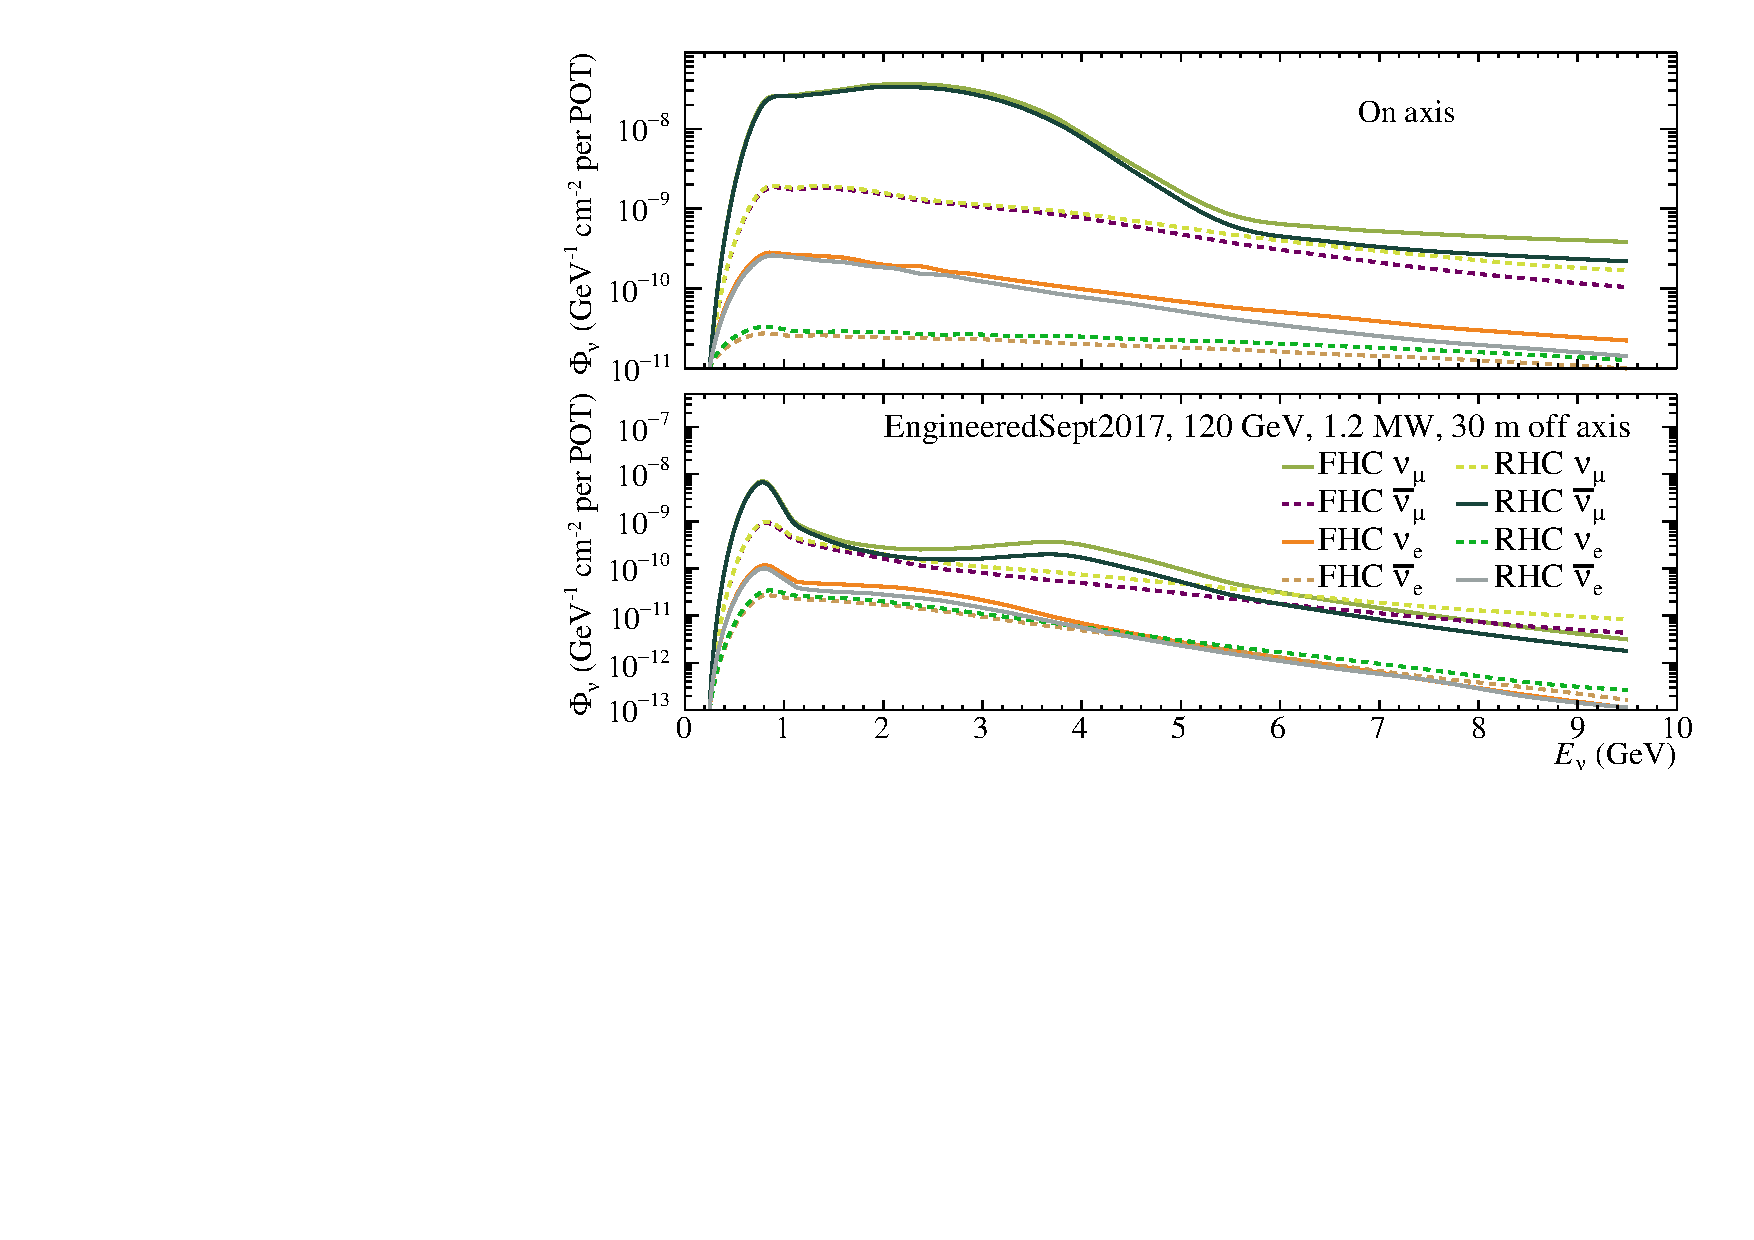
\includegraphics[width=0.8\textwidth]{OffAxisFluxes_1D_AllSpec}
    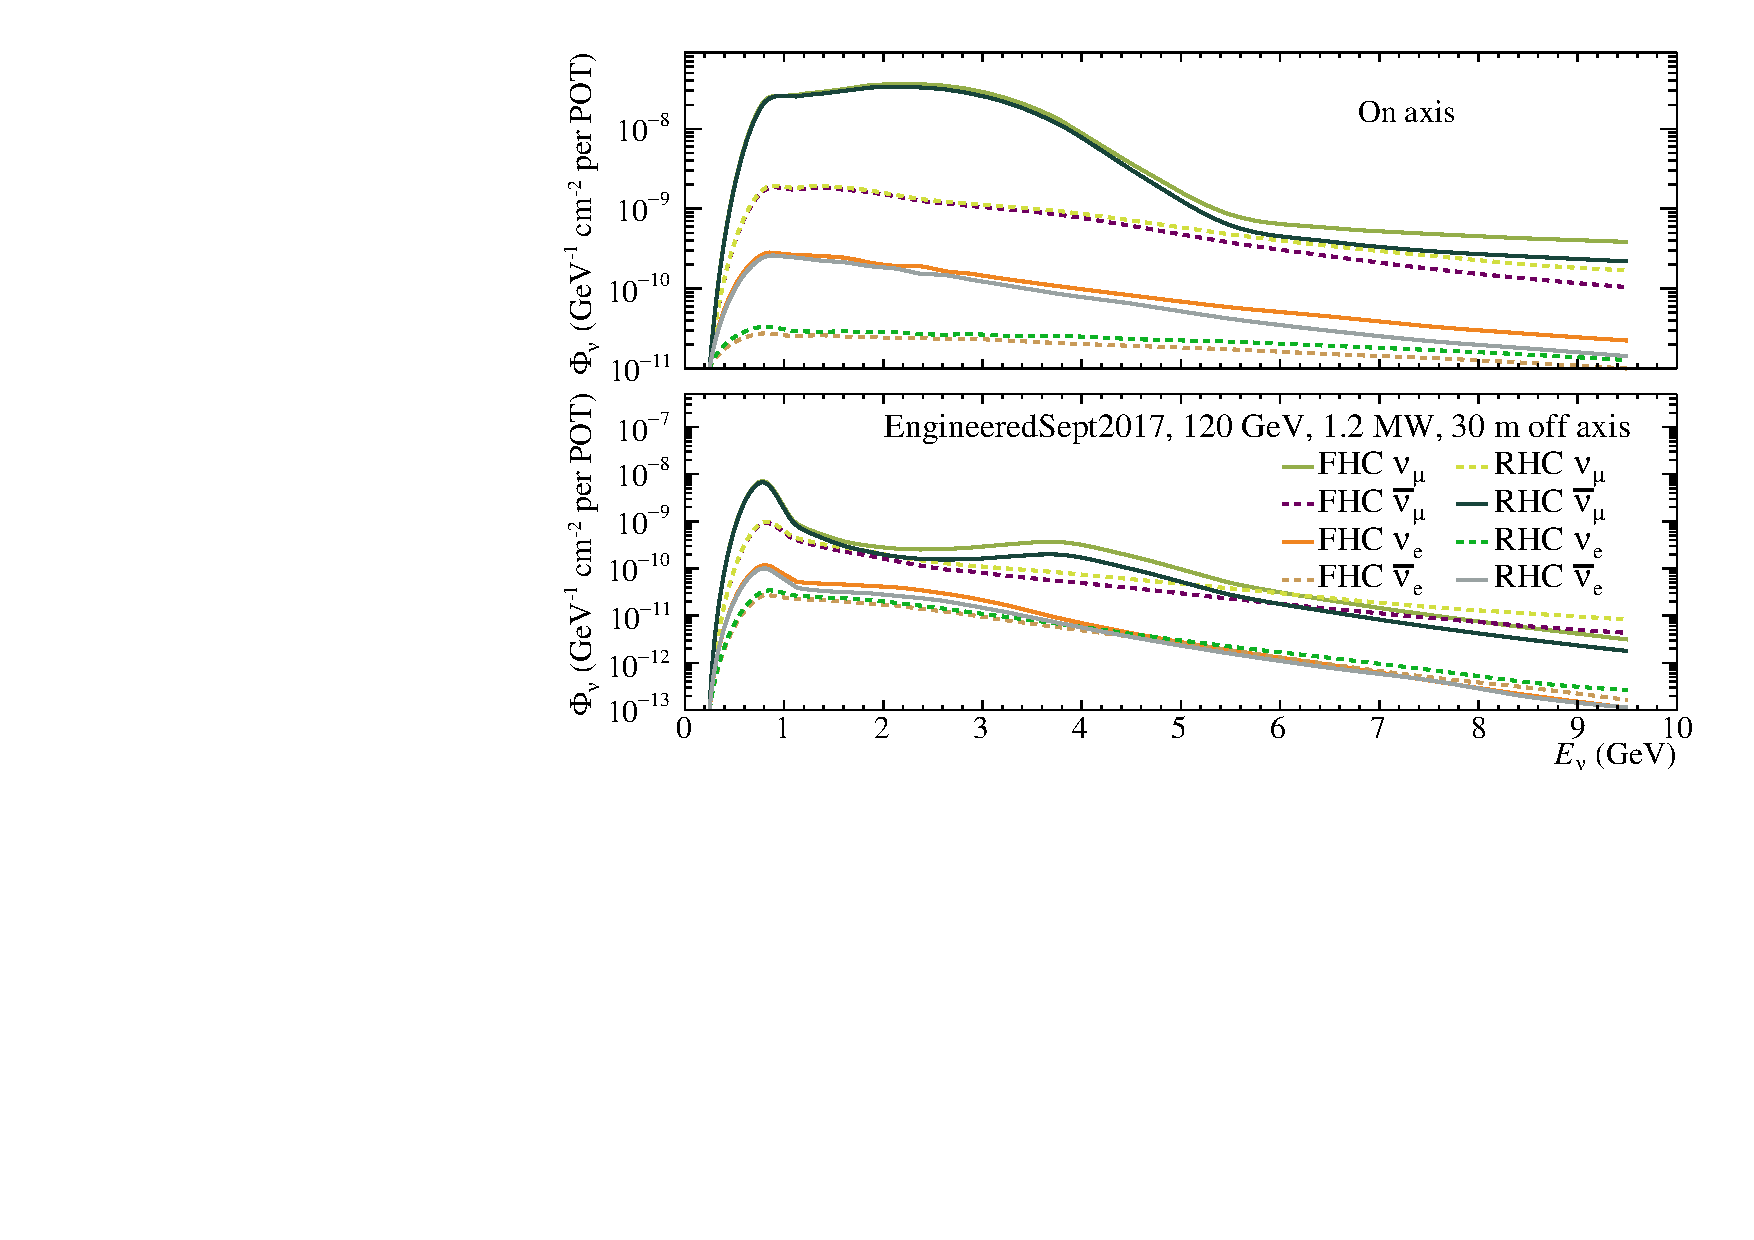
\includegraphics[width=0.8\textwidth]{OffAxisFluxes_1D_AllSpec}
  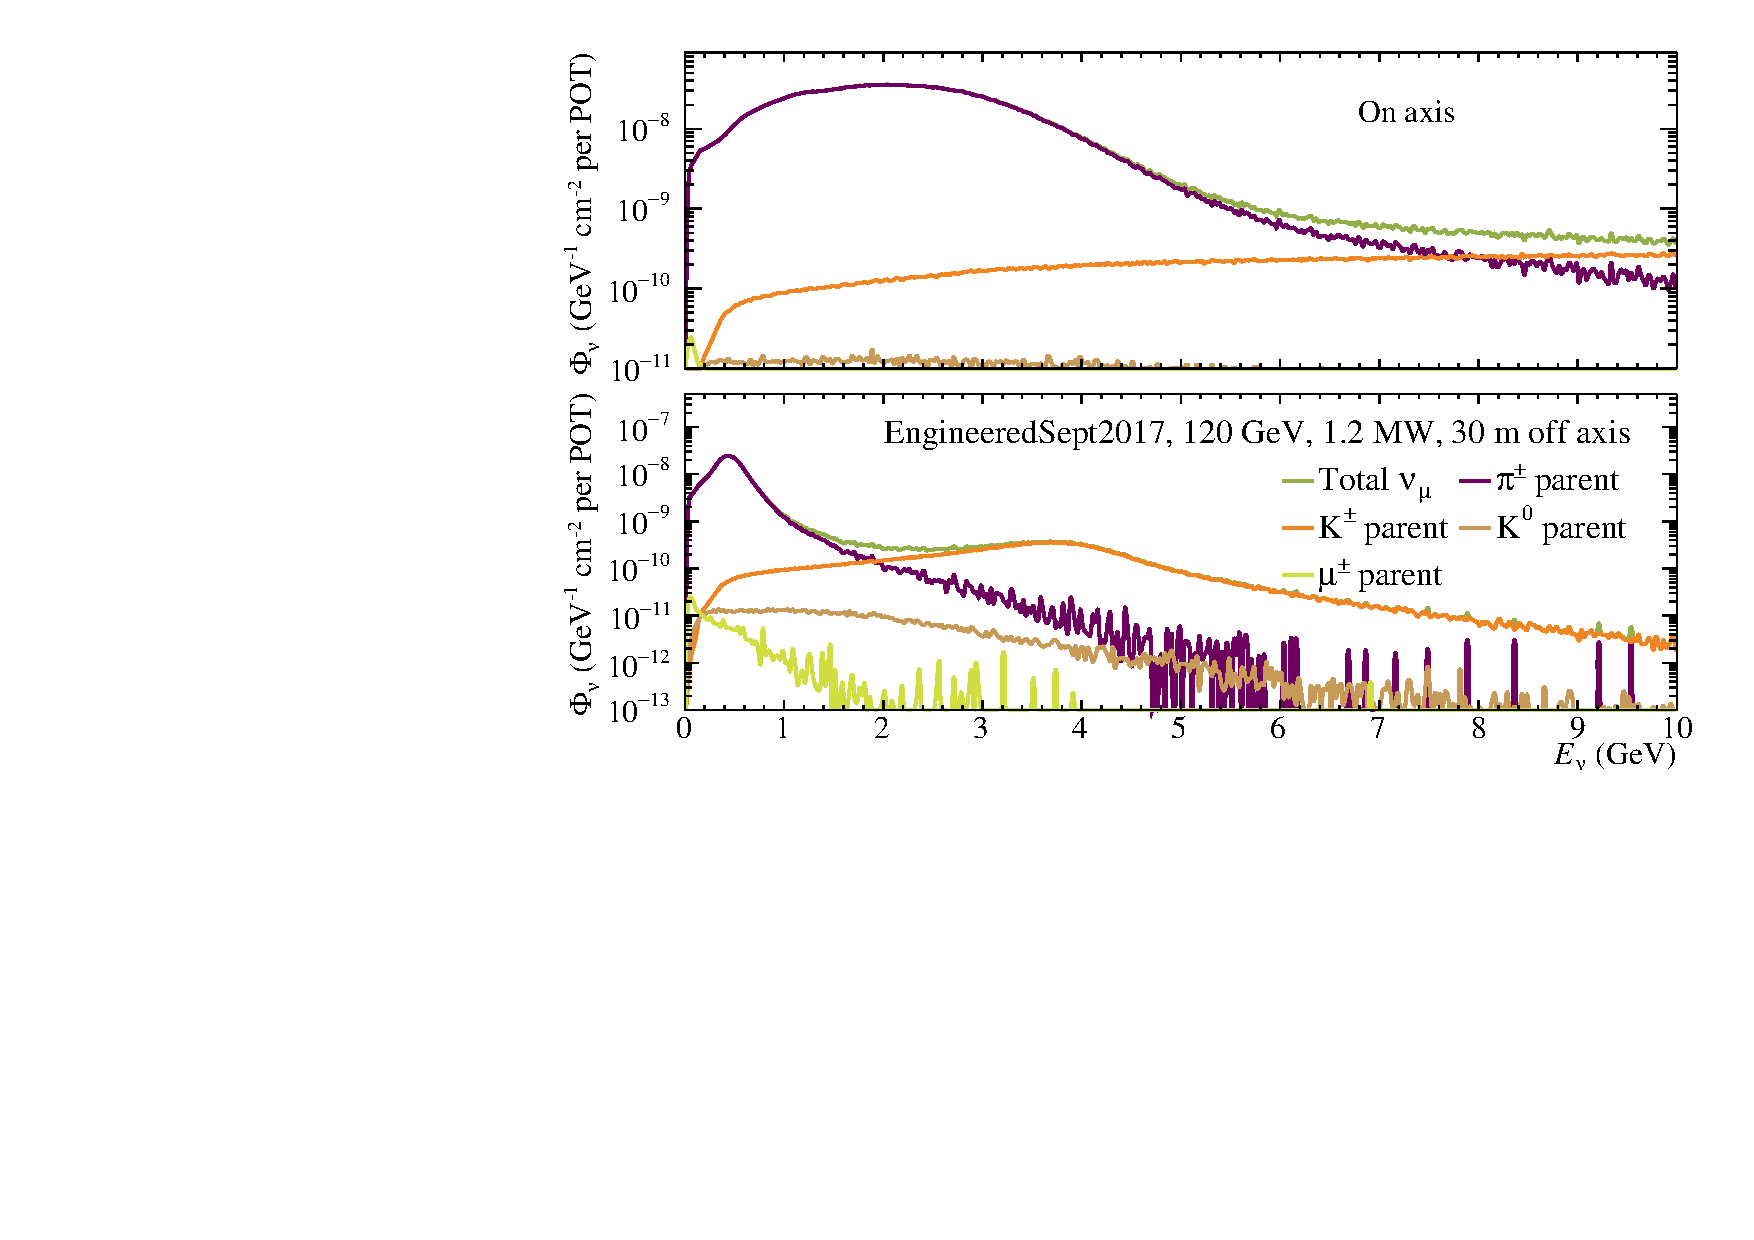
\includegraphics[width=0.8\textwidth]{OffAxisFluxes_1D_Parents}    
    \end{dunefigure}

%\fixme{one label per dunefigure; I didn't use label fig:OffAxisFluxes\_1D\_Parents or fig:OAAFluxFigsDetail - may need to fix refs}
%ZP: not sure what was the issue. looks fine to me now

The same sources of systematic uncertainty that affect the on-axis spectra also modify the off-axis spectra. 
Figure \ref{fig:onvsoff_flux_uncertainty} shows the on-axis and off-axis hadron production and focusing uncertainties. 
Generally, the size of the off-axis uncertainties is comparable to the on-axis uncertainties and the uncertainties are highly correlated across off-axis and on-axis positions. While the hadron production uncertainties are similar in size, the focusing uncertainties, are smaller for the off-axis flux. The systematic effects have different shape as function of neutrino energy at different off-axis locations making off-axis flux measurements useful to diagnose beamline physics. Measuring on-axis and off-axis flux breaks degeneracy between various systematics and allows better flux constraint.

%\fixme{DISCUSS FIGURE: Plot of extreme off-axis angle 1D uncertainty profiles? Can be relative off-axis to on-axis or just off-axis only. }

\begin{dunefigure}[On-axis and off-axis flux uncertainties]{fig:onvsoff_flux_uncertainty}
{The flux uncertainty for the on-axis flux, and several off-axis positions. Shown is the total hadron production uncertainty and several major focusing uncertainties.}
    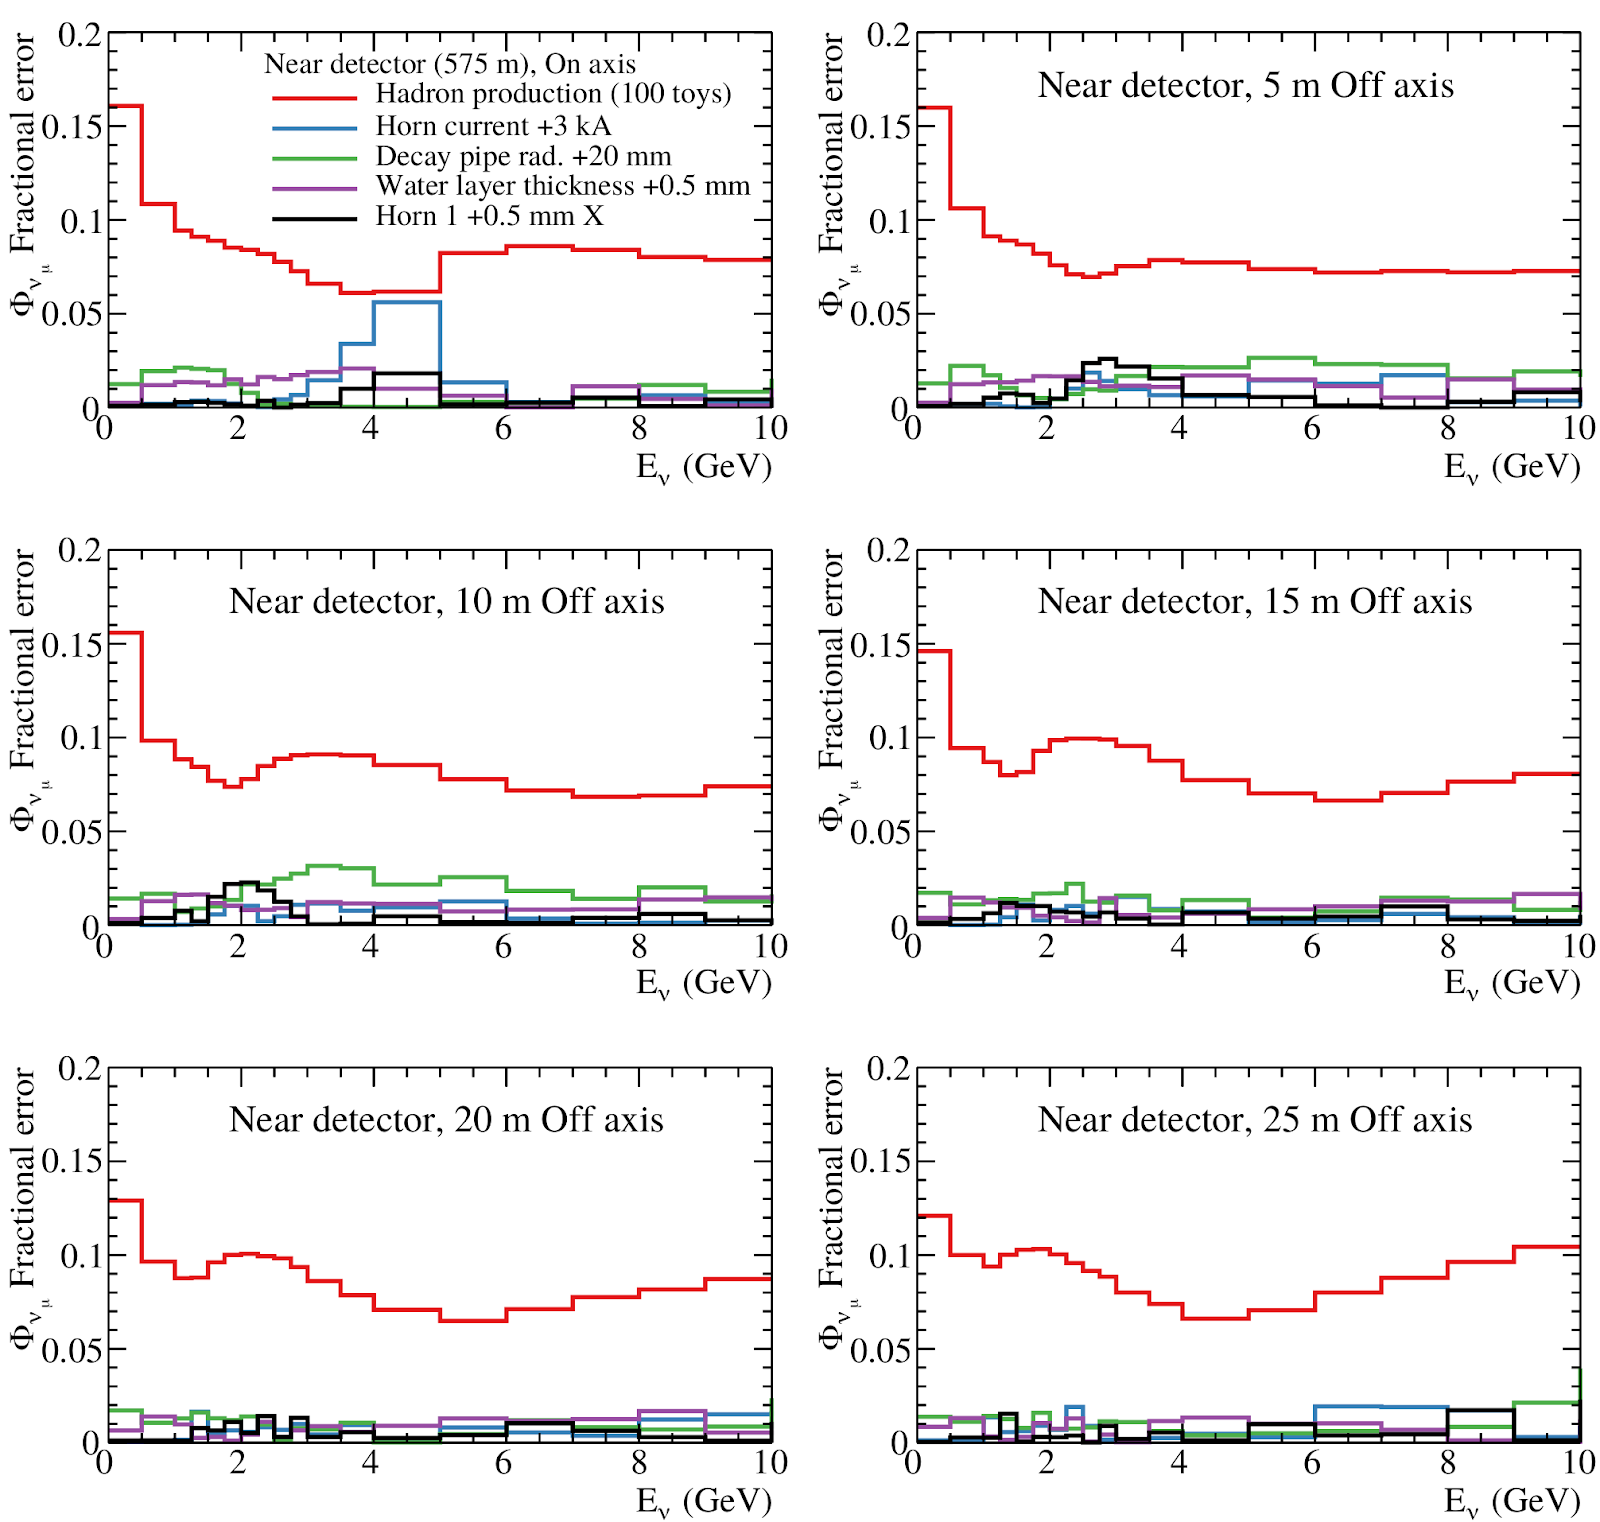
\includegraphics[width=0.8\textwidth]{graphics/onaxis_vs_offaxis_uncertainties.png}
\end{dunefigure}

%%%%%%%%%%%%%%%%%%%%%%%%%%%%%%%%%%%%%%%%%%%%%%%%%%%%%%%
\subsubsection{Additional Physics Generator Details}
\label{sec:tools-app-generator}

\paragraph{Nucleon Decay Channels}

The nucleon decay channels simulated by \dword{genie} are listed in Table~\ref{tab:genie_ndk}.
%while those used in the simulation of neutron-antineutron oscillations are given in 
%Table~\ref{tab:genie_antineutron}.

%\fixme{ TODO: replace raster version - was in table \ref{costas_table1} caption}
\begin{table}
  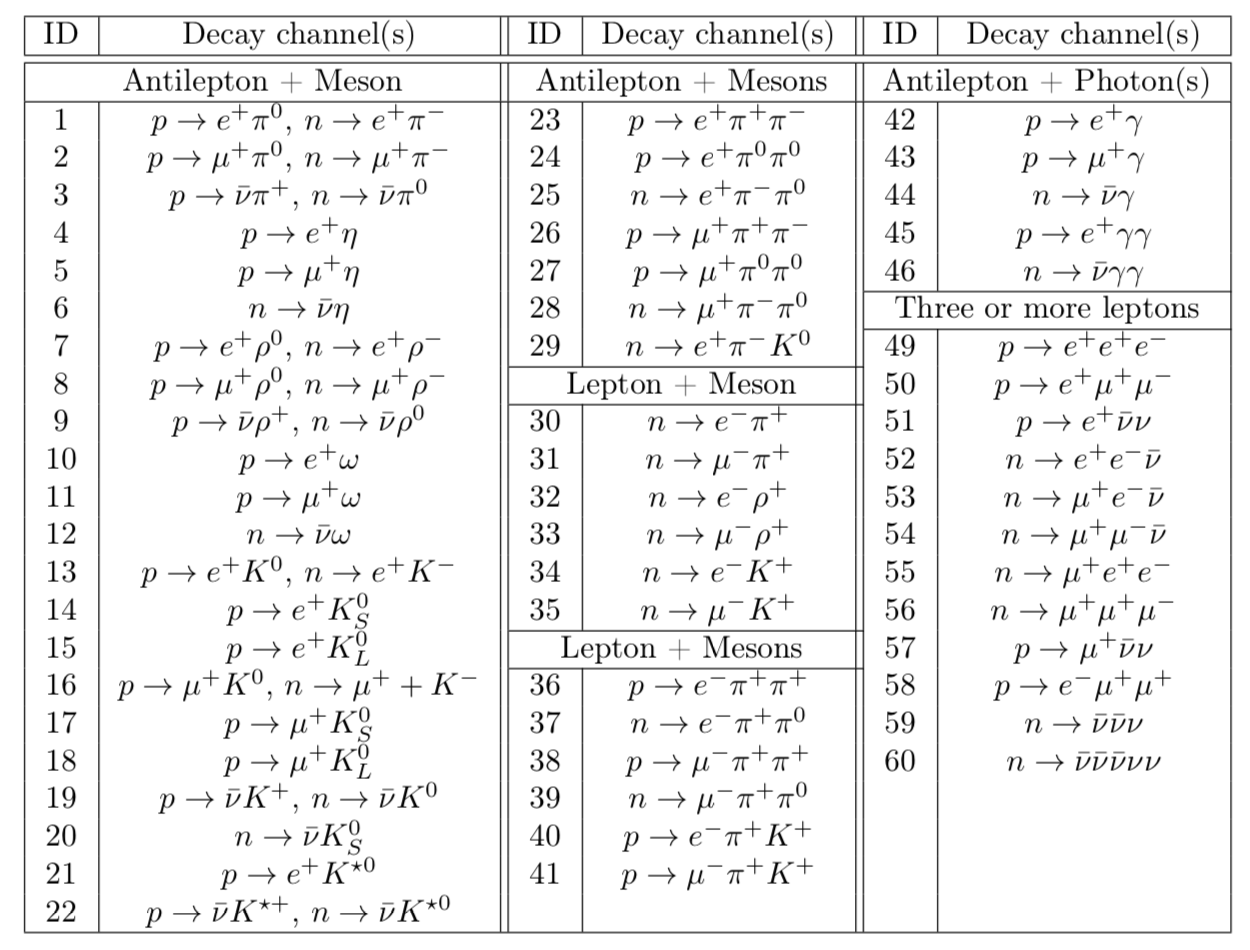
\includegraphics[width=\linewidth]{costas_table1}
  
  \caption[\dword{genie} nucleon decay topologies]{Decay topologies considered in \dword{genie} nucleon decay simulation.}
  \label{tab:genie_ndk}
\end{table}












